
\documentclass[dvipdfmx,uplatex,papersize,twoside,a5j,9pt,openright]{jsbook}
% %% fixes to LaTeX2e
% \usepackage{fix-cm}[2006/09/13 v1.1m]
% \usepackage{fixltx2e}[2006/09/13 v1.1m]


%% copy values from 'config-starter.yml'
\makeatletter
\def\starter@target{pbook}
\def\starter@draft{}
\def\starter@chapter@decoration{none}
\def\starter@chapter@align{left}
\def\starter@chapter@oneline{Y}
\def\starter@section@newpage{Y}
\def\starter@section@notopmargin{Y}
\def\starter@section@decoration{underline}
\def\starter@subsection@decoration{none}
\def\starter@caption@small{Y}
\def\starter@caption@pretty{Y}
\def\starter@program@fontsize{small}
\def\starter@terminal@fontsize{small}
\def\starter@program@ttfont{beramono}
\def\starter@terminal@ttfont{inconsolata}
\def\starter@colophon@poweredby{Y}
\makeatother


%% environment values for Starter
\makeatletter
\makeatother

\usepackage{mytextsize}

\usepackage[deluxe,uplatex]{otf}
\usepackage{caption}
\usepackage{suffix}
\usepackage[T1]{fontenc}\usepackage{textcomp}%T1/TS1
\usepackage{lmodern}
\usepackage[dvipdfmx]{graphicx}
\usepackage[dvipdfmx,table]{xcolor}%requires colortbl, array
\usepackage{framed}
\usepackage{wrapfig}
\definecolor{shadecolor}{gray}{0.9}
\definecolor{shadecolorb}{gray}{0.1}
\definecolor{reviewgreen}{rgb}{0,0.4,0}
\definecolor{reviewblue}{rgb}{0.2,0.2,0.4}
\definecolor{reviewred}{rgb}{0.7,0,0}
\definecolor{reviewdarkred}{rgb}{0.3,0,0}
\usepackage[utf8]{inputenc}
\usepackage{ascmac}
\usepackage{float}
\usepackage{alltt}
\usepackage{amsmath}

%% if you use @<u>{} (underline), use jumoline.sty
\IfFileExists{jumoline.sty}{
\usepackage{jumoline}
}

\newenvironment{shadedb}{%
  \def\FrameCommand{\fboxsep=\FrameSep \colorbox{shadecolorb}}%
  \MakeFramed {\FrameRestore}}%
 {\endMakeFramed}

%\usepackage[top=10zw,bottom=12zw,left=10zw,right=10zw]{geometry}
%\usepackage[top=5zw,bottom=5zw,left=1zw,right=1zw]{geometry}

\newcommand{\parasep}{\vspace*{3zh}}
\setlength{\footskip}{30pt}

%% Bookmarkの文字化け対策(日本語向け)
\usepackage[dvipdfmx,bookmarks=true,bookmarksnumbered=true,colorlinks=true,%
     pdftitle={Nuxt.jsとFirebase
でつくるアルゴリズム
ミニアプリ},%
     pdfauthor={pco2699}]{hyperref}
\usepackage[dvipdfmx]{pxjahyper}



\newenvironment{reviewimage}{%
  \begin{figure}[H]
    \begin{center}}{%
    \end{center}
  \end{figure}}

\newenvironment{reviewdummyimage}{%
  \begin{figure}[H]
    \begin{center}\begin{alltt}}{%
    \end{alltt}\end{center}
  \end{figure}}

\newcommand{\reviewimagecaption}[1]{%
  \caption{#1}}

\newenvironment{reviewemlist}{%
  \medskip\small\begin{shaded}\setlength{\baselineskip}{1.3zw}\begin{alltt}}{%
  \end{alltt}\end{shaded}}

\newenvironment{reviewlist}{%
  \begin{shaded}\small\setlength{\baselineskip}{1.3zw}\begin{alltt}}{%
  \end{alltt}\end{shaded}\par\vspace*{0.5zw}}

\newenvironment{reviewsource}{%
  \begin{shaded}\small\setlength{\baselineskip}{1.3zw}\begin{alltt}}{%
  \end{alltt}\end{shaded}\par\vspace*{0.5zw}}

\newenvironment{reviewcmd}{%
  \color{white}\medskip\small\begin{shadedb}\setlength{\baselineskip}{1.3zw}\begin{alltt}}{%
  \end{alltt}\end{shadedb}}

\newenvironment{reviewbox}{%
  \medskip\small\begin{framed}\setlength{\baselineskip}{1.3zw}\begin{alltt}}{%
  \end{alltt}\end{framed}}

\newenvironment{reviewtable}[1]{%
  \begin{center}\small\setlength{\baselineskip}{1.2zw}
    \begin{tabular}{#1}}{%
    \end{tabular}
  \end{center}}

\newenvironment{reviewcolumn}{%
     \begin{framed}
  }{%
     \end{framed}
  \vspace{2zw}}

\newcommand{\reviewcolumnhead}[2]{%
{\noindent\large ■コラム: #2}}

\newcommand{\reviewtablecaption}[1]{%
  \caption{#1}}

\WithSuffix\newcommand\reviewtablecaption*[1]{%
  \caption*{#1}}

\newcommand{\reviewimgtablecaption}[1]{%
  \caption{#1}\vspace{-3mm}}

\newcommand{\reviewbackslash}[0]{%
  \textbackslash{}}

\newcommand{\reviewlistcaption}[1]{%
  \medskip{\small\noindent #1}\vspace*{-1.3zw}}

\newcommand{\reviewemlistcaption}[1]{%
  \medskip{\small\noindent #1}\vspace*{-1.3zw}}

\newcommand{\reviewsourcecaption}[1]{%
  \medskip{\small\noindent #1}\vspace*{-1.3zw}}

\newcommand{\reviewcmdcaption}[1]{%
  \medskip{\small\noindent #1}\vspace*{-1.3zw}}

\newcommand{\reviewindepimagecaption}[1]{%
  \begin{center}#1\end{center}}

\newcommand{\reviewboxcaption}[1]{%
  \medskip{\small\noindent #1}\vspace*{-1.3zw}}

\newcommand{\reviewimageref}[2]{図 #1}
\newcommand{\reviewtableref}[2]{表 #1}
\newcommand{\reviewlistref}[1]{リスト #1}
\newcommand{\reviewbibref}[2]{#1}
\newcommand{\reviewcolumnref}[2]{コラム #1}
\newcommand{\reviewsecref}[2]{#1}

\newcommand{\reviewminicolumntitle}[1]{%
  {\large ■メモ: #1}\\}

\renewcommand{\contentsname}{目次}

\newenvironment{reviewminicolumn}{%
  \vspace{1.5zw}\begin{screen}}{%
  \end{screen}\vspace{2zw}}

\newcommand{\reviewkw}[1]{\textbf{\textgt{#1}}}
\newcommand{\reviewami}[1]{\mask{#1}{A}}
\newcommand{\reviewem}[1]{\textbf{#1}}
\newcommand{\reviewstrong}[1]{\textbf{#1}}
\newcommand{\reviewunderline}{\Underline}

%% @<del> is ignored in LaTeX with default style
\newcommand{\reviewstrike}[1]{#1}

%%%% for ulem.sty:
%%\renewcommand{\reviewstrike}[1]{\sout{#1}}
%%
%%%% for jumoline.sty:
%%\renewcommand{\reviewstrike}[1]{\Middleline{#1}}

\newcommand{\reviewth}[1]{\textgt{#1}}
\newcommand{\reviewtitlefont}[0]{\usefont{T1}{phv}{b}{n}\gtfamily}
\newcommand{\reviewmainfont}[0]{}
\newcommand{\reviewcolophon}[0]{\clearpage}
\newcommand{\reviewappendix}[0]{\appendix}

\newcommand{\reviewprepartname}{第}
\newcommand{\reviewpostpartname}{部}
\newcommand{\reviewprechaptername}{第}
\newcommand{\reviewpostchaptername}{章}
\newcommand{\reviewfigurename}{図}
\newcommand{\reviewtablename}{表}
\newcommand{\reviewappendixname}{付録}

\ifdefined\prepartname
  \renewcommand{\prepartname}{\reviewprepartname}
\fi
\ifdefined\postpartname
  \renewcommand{\postpartname}{\reviewpostpartname}
\fi
\ifdefined\prechaptername
  \renewcommand{\prechaptername}{\reviewprechaptername}
\fi
\ifdefined\postchaptername
  \renewcommand{\postchaptername}{\reviewpostchaptername}
\fi
\ifdefined\figurename
  \renewcommand{\figurename}{\reviewfigurename}
\fi
\ifdefined\tablename
  \renewcommand{\tablename}{\reviewtablename}
\fi
\ifdefined\appendixname
  \renewcommand{\appendixname}{\reviewappendixname}
\fi


\makeatletter
%% maxwidth is the original width if it is less than linewidth
%% otherwise use linewidth (to make sure the graphics do not exceed the margin)
\def\maxwidth{%
  \ifdim\Gin@nat@width>\linewidth
    \linewidth
  \else
    \Gin@nat@width
  \fi
}

\makeatother

\usepackage{reviewmacro}
\usepackage{starter}
\usepackage{mystyle}
\usepackage{mytitlepage}
\usepackage{mycolophon}

\begin{document}

\reviewmainfont

%%%
\title{Nuxt.jsとFirebase\\
でつくるアルゴリズム\\
ミニアプリ}
\makeatletter
\def\@subtitle{}
\def\@pubevent{技術書典7(2019年秋)新刊}
\def\@latestpubhistory{2019年9月22日 ver 1.0}
\makeatother
\author{pco2699 著}
\date{2019{-}09{-}22 版\hspace{2zw} 発行}
%%%
\begin{titlepage}
  \ifdefined\mytitlepage %%%%%%%%%%
    \mytitlepage   % defined in 'sty/mytitlepage.sty'
  \else                  %%%%%%%%%%
\thispagestyle{empty}
\begin{center}%
  \mbox{} \vskip5zw
   \reviewtitlefont%
    {\HUGE\bfseries Nuxt.jsとFirebase
でつくるアルゴリズム
ミニアプリ \par}%
    \vskip 1em%
    {\Large {\rmfamily --- }  {\rmfamily --- } \par}%
    \vskip 15em%
    {\LARGE
      \lineskip .75em
      \begin{tabular}[t]{c}%
        pco2699 著
      \end{tabular}\par}%
    \vfill
    {\large 2019{-}09{-}22 版\hspace{2zw} 発行\par}%
\vskip4zw\mbox{}
  \end{center}%
  \fi                    %%%%%%%%%%
\end{titlepage}
\ifdefined\mytitlenextpage
  \mytitlenextpage
\fi

%\renewcommand{\chaptermark}[1]{{}}
\frontmatter

%%% originaltitle

%%% credit

%% preface
\chapter{まえがき}
\label{chap:chap00-preface}

\section*{自己紹介}
\addcontentsline{toc}{section}{自己紹介}
\label{sec:-1}

はじめまして、こんにちは、たかやま(@pco2699)と申します。
普段は、資産運用のスタートアップでJavaのバックエンドエンジニアとして働いています。

土日は、ハッカソンに出たり、このようなちょっとしたアプリをつくるような開発本を書いたり
プチ0{-}\textgreater{}1を楽しむのが、日課です。

\section*{Webエンジニアにアルゴリズム/データ構造の知識は必要か}
\addcontentsline{toc}{section}{Webエンジニアにアルゴリズム/データ構造の知識は必要か}
\label{sec:-2}

よくはてぶのホッテントリやTwitterでも話題に上がる、\textbf{Webエンジニアにアルゴリズム・データ構造などの知識は必要か?}論。
皆さんも目にしたことがあると思います。この論について、どのような意見をお持ちでしょうか?

私、個人としては、\textbf{無くても困らないけど、あると色々助かる。}ものだと思っています。
こういったCS(コンピュータ・サイエンス)と呼ばれる以下のような知識は、エンジニアにとっては\textbf{筋肉}のようなものだと思います。

\begin{starteritemize}
\item アルゴリズム
\item データ構造
\item ネットワーク
\item オペレーティング・システム
\end{starteritemize}

などなど...

筋肉ももちろん無くて困ることはありませんが、あるといろいろ便利です。

\section*{でも、アルゴリズムの勉強って何に使うの??}
\addcontentsline{toc}{section}{でも、アルゴリズムの勉強って何に使うの??}
\label{sec:-3}

Webエンジニアとして働いていると、もちろんアルゴリズムがそのまま出てくることなんて、そうそう無いです。
普通にWebページを作る、ということであれば、アルゴリズムの知識なんて全然使わないと思います。

しかも、町の本屋さんやAmazonで売っているいわゆる「アルゴリズム・データ構造」が載っている本は
ストイックにアルゴリズムやデータ構造が書いてあるので、まあ読む気が失せるわけです。

そこで、私はアルゴリズムをそのまま小さいWebアプリ = アルゴリズムミニアプリ として
実装することで、「アルゴリズムがWebアプリでどのように活かされるか」をわかりやすく理解できる本を書きたいと思いました。

それが本書「Nuxt.jsとPythonでつくるアルゴリズムミニアプリ」です。

\section*{アルゴリズムミニアプリってなに?}
\addcontentsline{toc}{section}{アルゴリズムミニアプリってなに?}
\label{sec:-4}

「アルゴリズムミニアプリってなんだろう」と思う方もいると思います。
アルゴリズムミニアプリは、以下の要素をもつWebアプリです。(この概念自体はもちろん、自分が作ったものです。)

\begin{starteritemize}
\item Facebookの友達検索機能!など、Webサービスの一つの機能だけをアプリとして切り出したもの。
\item ゲーム好きの方なら「メイドインワリオ」のWebサービス 
\end{starteritemize}

\section*{対象読者}
\addcontentsline{toc}{section}{対象読者}
\label{sec:-5}

本書の対象読者は以下のような方です。
特に1.の方を対象としています。

\begin{starterenumerate}
\item アルゴリズムがよくわからないWeb系のエンジニア
\item アルゴリズムがどのようにWebアプリに活用されるか知りたい人
\item CS専攻で、モダンなWeb技術でのアプリの技術スタック、開発方法が知りたい人
\end{starterenumerate}

言語はJavaScriptをメインで利用します。
JavaScriptを書いたことが無くても、C, C++, Java, Python, Ruby, PHPなどの言語をどれか一つで
簡単なWebシステムやツールを書いたことがある方なら理解できる内容となっていると思います。

逆に以下のような方は、本書を読んでも??となってしまうかもしれません。

\begin{starterenumerate}
\item プログラミングを全くしたことが無い方
\end{starterenumerate}

\section*{本書の構成}
\addcontentsline{toc}{section}{本書の構成}
\label{sec:-6}

本書は、各章で一つのアルゴリズムを取り上げます。
章の前半でアルゴリズムの解説、後半でWebアプリの説明、およびコード内容の説明を行います。



\setcounter{tocdepth}{2}
\tableofcontents

%\renewcommand{\chaptermark}[1]{\markboth{\prechaptername\thechapter\postchaptername~#1}{}}
\mainmatter
\chapter{環境構築}
\label{chap:chap01-install}

各種アルゴリズムの説明に入る前に、今回作成するWebアプリの基本構成および環境構築の方法について説明します。

各章でそれぞれ一つのミニアプリを作る予定ですが、すべて同じ環境上に作るため、ここでまとめて説明します。

\section{今回の構成}
\label{sec:1-1}

今回は以下の構成でWebアプリを作ります。

\begin{reviewimage}%%architecture
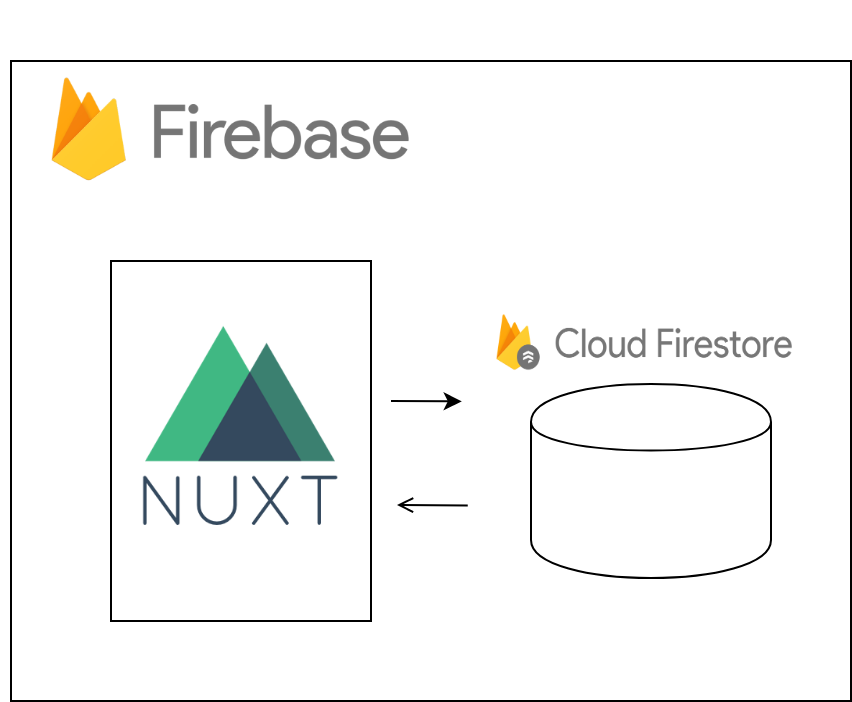
\includegraphics[width=\maxwidth]{./images/architecture.png}%
\reviewimagecaption{今回の構成}
\label{image:chap01-install:architecture}
\end{reviewimage}

それぞれの要素について説明します。

\subsection*{Firebase}
\addcontentsline{toc}{subsection}{Firebase}
\label{sec:1-1-1}

今回は、Firebaseと呼ばれるWebサイトのホスティングやDBをサクッと作れるBaaS(Backend as a service)上にWebサービスを作ります。
Firebaseを利用することで、難しかったインフラ構築やサーバーデプロイなどの作業が不要になるため、一人でWebサービスをサクッとプロトタイピングするのに向いています。

サクッと一人で、コストも抑えてWebアプリを作るため、Firebaseを今回は採用することにしました。

\subsection*{Firebase Hosting}
\addcontentsline{toc}{subsection}{Firebase Hosting}
\label{sec:1-1-2}

Firebase HostingはFirebaseのサービスの一つで、HTMLやCSS、JSなどの静的ファイルをホスティングするためのサービスです。
PHPやJava, Pythonなどはもちろん動きませんが、後述する「静的サイトジェネレーター」を組み合わせることで、フロントエンドフレームワークで作成された
ファイルをデプロイすることができます。

コストも抑えることができるので、個人開発などにおすすめです。

\subsection*{Cloud Firestore}
\addcontentsline{toc}{subsection}{Cloud Firestore}
\label{sec:1-1-3}

データの永続化を行うDBです。少し前のWebサービスだと \texttt{MySQL}や」

\subsection*{Nuxt.js}
\addcontentsline{toc}{subsection}{Nuxt.js}
\label{sec:1-1-4}

今回、Nuxt.jsと呼ばれるフロントエンドフレームワークを用いて、Webサービスを作成します。Nuxt.jsはVue.jsと呼ばれるフレームワークはベースになっており
HTML/CSSが理解できていれば、非常に理解しやすく扱いやすいフロントエンドフレームワークです。

Nuxt.jsには「静的サイトジェネレーター」の機能もあり、これを用いて、生成されたHTML/CSSなどを firebase hostingにデプロイすることで
今回のWebアプリを作っていきます。

\subsection*{Cloud Firestore}
\addcontentsline{toc}{subsection}{Cloud Firestore}
\label{sec:1-1-5}

\section{環境をつくろう}
\label{sec:1-2}

\subsection*{Firebaseへのサインアップ}
\addcontentsline{toc}{subsection}{Firebaseへのサインアップ}
\label{sec:1-2-1}

\subsection*{Nuxt.jsの導入}
\addcontentsline{toc}{subsection}{Nuxt.jsの導入}
\label{sec:1-2-2}

\chapter{探索}
\label{chap:chap02-search}

では、早速アルゴリズムを学んでいきましょう!
一番、最初は、最も基礎である「探索」を学びます!

\section{アルゴリズムの説明}
\label{sec:2-1}

\section{作るアプリ}
\label{sec:2-2}

\section{Webアプリのコード説明}
\label{sec:2-3}

\chapter{ソート}
\label{chap:chap03-sort}

\section{アルゴリズムの説明}
\label{sec:3-1}

\subsection*{バブルソート}
\addcontentsline{toc}{subsection}{バブルソート}
\label{sec:3-1-1}

\section{作るアプリ}
\label{sec:3-2}

\section{Webアプリのコード説明}
\label{sec:3-3}

\chapter{ヒープ/二分探索木}
\label{chap:chap04-heap}

\section{アルゴリズムの説明}
\label{sec:4-1}

\section{作るアプリ}
\label{sec:4-2}

\section{Webアプリのコード説明b}
\label{sec:4-3}

\chapter{動的計画法}
\label{chap:chap05-dp}

\section{アルゴリズムの説明}
\label{sec:5-1}

\subsection*{バブルソート}
\addcontentsline{toc}{subsection}{バブルソート}
\label{sec:5-1-1}

\section{作るアプリ}
\label{sec:5-2}

\section{Webアプリのコード説明}
\label{sec:5-3}


%\renewcommand{\chaptermark}[1]{\markboth{\appendixname\thechapter~#1}{}}
\reviewappendix


%% backmatter begins
\backmatter

\chapter{あとがき}
\label{chap:chap99-afterword}



%%% profile

%%% advfile

%%% colophon
%% okuduke
\ifdefined\mycolophon  %%%%%%%%%%
  \title{Nuxt.jsとFirebase
でつくるアルゴリズム
ミニアプリ}
  \makeatletter
  \def\@subtitle{}
  \makeatother
  \def\colophonpubhistory{%
    2019年9月22日 ver 1.0%
  }
  \def\colophonokuduke{%
    著 者 & pco2699 \\
印刷所 & 日光企画 \\
%
  }
  \def\colophonrights{%
    
    {\textcopyright} 2019 pco2699\\
    
  }
  \mycolophon     % defined in 'sty/mycolophon.sty'
\else                  %%%%%%%%%%
\reviewcolophon
\thispagestyle{empty}

\vspace*{\fill}

{\noindent\reviewtitlefont\Large Nuxt.jsとFirebase
でつくるアルゴリズム
ミニアプリ} \\
\medskip
{\noindent\reviewtitlefont } \\
\rule[8pt]{\textwidth}{1pt} \\
{\noindent
2019年9月22日 ver 1.0
}
\medskip

\begin{tabular}{ll}
著 者 & pco2699 \\
印刷所 & 日光企画 \\

\end{tabular}
% \\

\medskip
\noindent
\rule[0pt]{\textwidth}{1pt} \\
(C) 2019 pco2699 \\
\fi                    %%%%%%%%%%

%%% backcover

\end{document}
